
\let\negmedspace\undefined
\let\negthickspace\undefined
\documentclass[journal]{IEEEtran}
\usepackage[a5paper, margin=10mm, onecolumn]{geometry}
%\usepackage{lmodern} % Ensure lmodern is loaded for pdflatex
\usepackage{tfrupee} % Include tfrupee package

\setlength{\headheight}{1cm} % Set the height of the header box
\setlength{\headsep}{0mm}     % Set the distance between the header box and the top of the text

\usepackage{gvv-book}
\usepackage{gvv}
\usepackage{cite}
\usepackage{amsmath,amssymb,amsfonts,amsthm}
\usepackage{algorithmic}
\usepackage{graphicx}
\usepackage{textcomp}
\usepackage{xcolor}
\usepackage{txfonts}
\usepackage{listings}
\usepackage{enumitem}
\usepackage{mathtools}
\usepackage{gensymb}
\usepackage{comment}
\usepackage[breaklinks=true]{hyperref}
\usepackage{tkz-euclide} 
\usepackage{listings}
% \usepackage{gvv}                                        
\def\inputGnumericTable{}                                 
\usepackage[latin1]{inputenc}                                
\usepackage{color}                                            
\usepackage{array}                                            
\usepackage{longtable}                                       
\usepackage{calc}                                             
\usepackage{multirow}                                         
\usepackage{hhline}                                           
\usepackage{ifthen}                                           
\usepackage{lscape}
\usepackage{circuitikz}
\tikzstyle{block} = [rectangle, draw, fill=blue!20, 
    text width=4em, text centered, rounded corners, minimum height=3em]
\tikzstyle{sum} = [draw, fill=blue!10, circle, minimum size=1cm, node distance=1.5cm]
\tikzstyle{input} = [coordinate]
\tikzstyle{output} = [coordinate]


\begin{document}

\bibliographystyle{IEEEtran}
\vspace{3cm}

\title{1.9.32}
\author{EE25BTECH11044 - Sai Hasini Pappula}
 \maketitle
% \newpage
% \bigskip
{\let\newpage\relax\maketitle}

\renewcommand{\thefigure}{\theenumi}
\renewcommand{\thetable}{\theenumi}
\setlength{\intextsep}{10pt} % Space between text and floats


\numberwithin{equation}{enumi}
\numberwithin{figure}{enumi}
\renewcommand{\thetable}{\theenumi}

\textbf{Question:}\\
If the distance between the points $(3,-5)$ and $(x,-5)$ is $15$ units, then find the values of $x$ using matrices.

\bigskip

\textbf{Solution:}\\
Let 
\[
\vec{A} = \begin{bmatrix} 3 \\ -5 \end{bmatrix}, 
\quad 
\vec{B} = \begin{bmatrix} x \\ -5 \end{bmatrix}.
\]

The distance between two points is given by
\[
d = \|\vec{B}-\vec{A}\|.
\]

So,
\[
d^2 = (\vec{B}-\vec{A})^{T}(\vec{B}-\vec{A}).
\]

Substituting,
\[
d^2 = 
\begin{bmatrix} x-3 \\ 0 \end{bmatrix}^{T}
\begin{bmatrix} x-3 \\ 0 \end{bmatrix}
= (x-3)^2.
\]

Given $d = 15$, we have
\[
(x-3)^2 = 225.
\]

Taking square roots,
\[
x-3 = \pm 15.
\]

Hence,
\[
x = 18 \quad \text{or} \quad x = -12.
\]

\begin{center}
    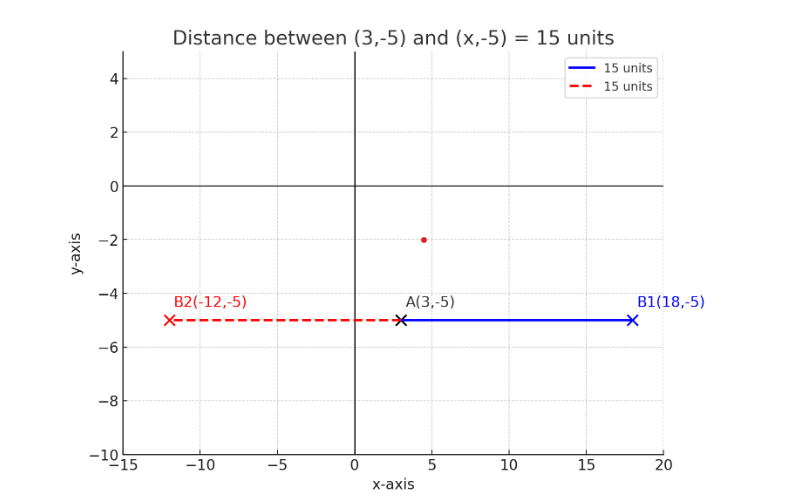
\includegraphics[width=0.6\columnwidth]{figs/plot2.png}
\end{center}

\end{document}
